

\section{Wednesday}\index{Wednesday_lecture}
\subsection{Three Examples}
\begin{example}[Chase problem]
A rabit starts at (0,0) and runs up  the y-axis with speed $a$ toward its burrow. A dog at the same time running with speed $b$ at (c,0) and persuit the rabbit. What is the path of the dog?\\
\begin{figure}[H]
\centering
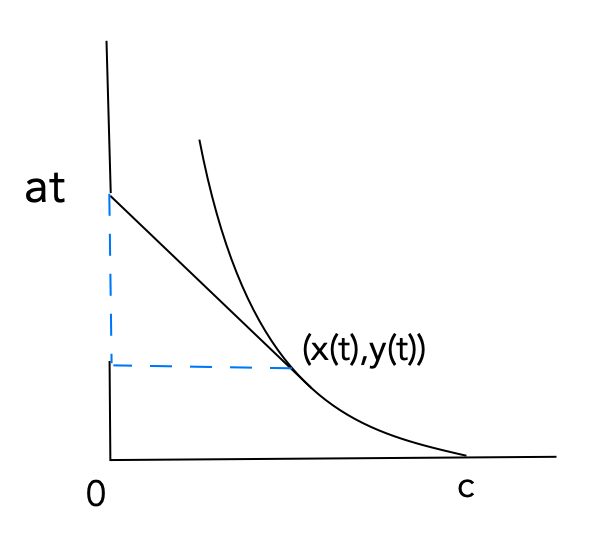
\includegraphics[width=6cm]{week4_wed}
\end{figure}
From the figure, we can get that;
\[\frac{\diff y}{\diff x}=-\frac{at-y(t)}{x(t)}
\]
By the way, all the following `` $^\prime$ '' will represent $\frac{\diff}{\diff x}$.\\
Rewrite it a little bit;
\[xy^\prime=y-at .
\]
Differentiate it with respect to x,
\[y^\prime+xy^{\prime\prime}=y^\prime-\frac{a\diff t}{\diff x}.
\]
Now, it seems there is a need to know more about $\frac{\diff t}{\diff x}$.\\
By calculus, we know the formula to compute the length of a curve:
\[S(x)=\int_x^c\sqrt{1+{y^{\prime}}^{2}}\diff x
\]
The speed of dog is the derivative of length it goes by time.
\[b=\frac{\diff s}{\diff t}=\frac{\diff s}{\diff x}\frac{\diff x}{\diff t}=-\sqrt{1+{y^{\prime}}^2}\frac{\diff x}{\diff t}\qquad\cdots(1)
\]
By (1), we know what is $\frac{\diff x}{\diff t}$. Pluge that in, we get.
\[xy^{\prime\prime}=\frac{a\sqrt{1+{y^{\prime}}^2}}{b}
\]
Set $z=y^\prime$, $r=\frac{a}{b}$, we rewrite the above equation.
\[xz^\prime=r\sqrt{1+z^2}
\]
God bless us that this is a first order linear differential equation we can solve.\\
By the way we solve seperable equation,
\[\int\frac{\diff z}{\sqrt{1+z^2}}=\int\frac{r}{x}\diff x
\]
With ingenious, skillful, and some how tedious substitution, i.e. $z=tan\theta$, $\diff z=\sec^2\theta\diff\theta$, the computation of left hand side can be managed. By the way, with this replacement, $1+z^2=1+\frac{\sin^2\theta}{\cos^2\theta}=\frac{1}{\cos^2\theta}=\sec^2\theta$
\[\int\frac{\diff z}{\sqrt{1+z^2}}=\int\frac{\sec^2\theta}{\sec}\diff\theta=\int\frac{1}{\cos\theta}\diff\theta=\int\frac{\cos\theta}{\cos^2\theta}\diff \theta=\int\frac{\diff\sin\theta}{1-\sin^2\theta}
\]
Again, with unspeakable thoughts, let $u=\sin\theta$, the above
\[=\int\frac{1}{1-u^2}\diff u=\int(\frac{\frac{1}{2}}{1-u}+\frac{\frac{1}{2}}{1+u})\diff u
\]
\[=\frac{1}{2}ln|\frac{1+u}{1-u}|+C=ln|\sec\theta+\tan\theta|+C
\]
This shows you why the last equal sign is the case.
\[\frac{1+\sin\theta}{1-\sin\theta}\frac{1+\sin\theta}{1+\sin\theta}=(\frac{1+\sin\theta}{\cos\theta})^2=(\sec\theta+\tan\theta)^2
\]
Now, with those details, we know why the seperable equation looks like this;
\[ln|z+\sqrt{1+z^2}|=rln|x|+C
.\]
\[|z+\sqrt{1+z^2}|=|x|^r\tilde{c}
\]
That is 
\[y^\prime+\sqrt{1+{y^\prime}^2}=\tilde{c}x^r.
\]
By observation,
\[y(s)=0=y^\prime(c).
\]
Therefore, $\tilde{c}=(\frac{1}{c})^r$.\\
Now, let's take square and then integrate $y^\prime$ to get what we want.\\
\[y^\prime+\sqrt{1+{y^\prime}^2}=(\frac{x}{c})^r
\]
\[1+{y^\prime}^2=(\frac{x}{c})^{2r}-2(\frac{x}{c})^ry^\prime+{y^\prime}^2
\]
\[\boxed{y^\prime=\frac{1}{2}(\frac{x}{c})^r-\frac{1}{2}(\frac{x}{c})^{-r}}
\]
$r$ is the rate of rabbit's speed verses dog's.\\
When $r=1$,
\[y=\frac{1}{2}\frac{1}{2}(\frac{x}{c})^2\cdot c-\boxed{\frac{c}{2}lnx}+C.
\]
When $r\neq1$,
\[y=\frac{1}{2}\frac{1}{c^r}\frac{1}{r+1}x^{r+1}-\frac{1}{2}c^r\frac{1}{1-r}x^{1-r}+C
\]
\end{example}
\begin{example}
Four bugs sit at the corners of a square table of side $a$. At the same time, they all begin to walk at the same speed, each moving steadily toward the bug to its right. Describe the path of the bugs. In addition, compute the length of the path.
\begin{figure}[H]
\centering
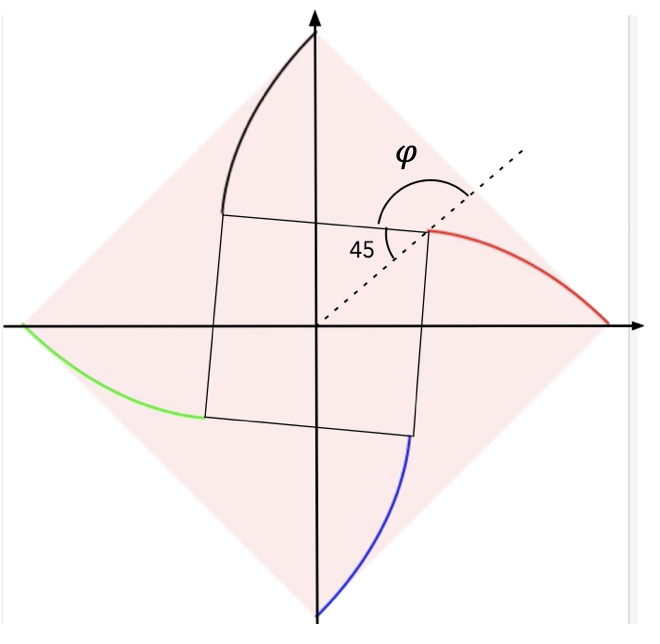
\includegraphics[width=8cm]{week4_bugs}
\caption{Pictures with further edition from; https://demonstrations.wolfram.com/FourBugProblem/}
\end{figure}
The ode knowledge used in this example is pretty trivial, that is, we use polar cordinate to illustrate the path with relation between $r$ (the length from the bug to origin) and $\theta$. However, before that, the relation between $r$ and $\theta$ need to be derived, i.e. the direvative of $r$ over $\theta$. (Why is this? Frankly, I don't know. Maybe, it is by experience.)\\
Now, let's have a look at detailed graph of the path in order to compute the derivative.
\begin{figure}[H]
\centering
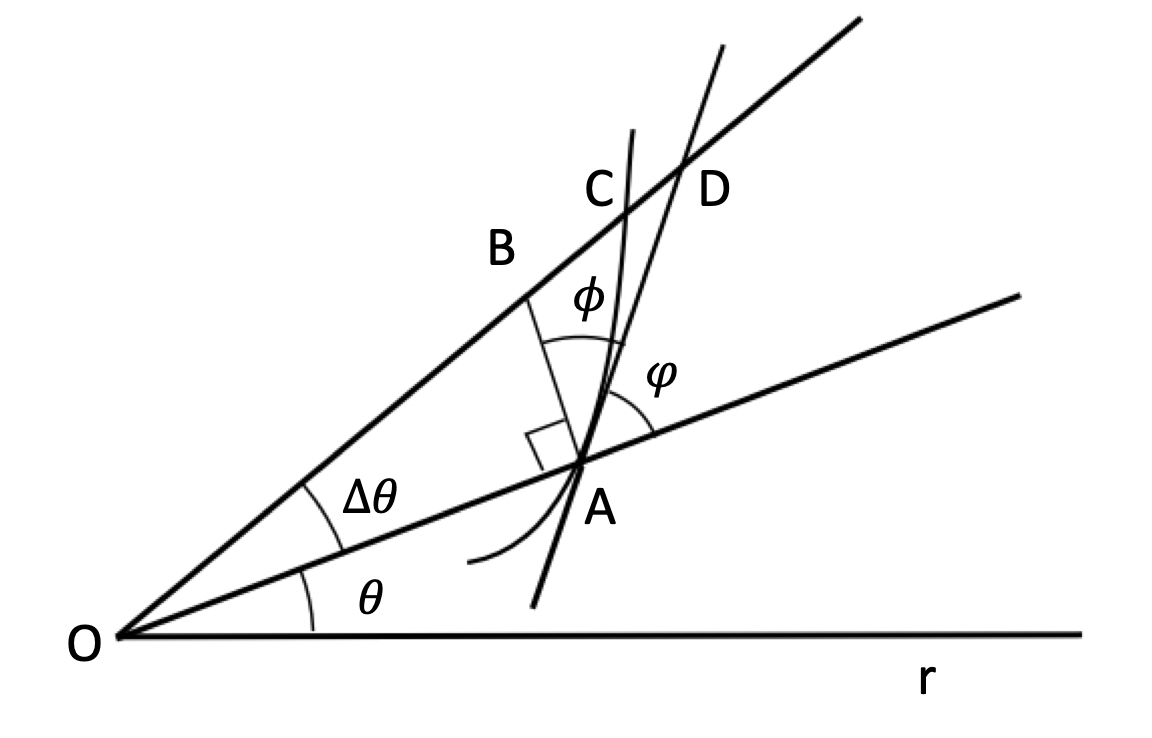
\includegraphics[width=10cm]{week4_r}
\end{figure}
In this graph, AC is the path that bug goes, AD is tangent line of AC at A, (r,$\theta$) is the polar cordinate. We know from figure 7.1 (see above) $\varphi=135^\circ$. $\tan\varphi=\cot\phi$. As $\Delta\theta$ is pretty small, $\cot\phi=\frac{AB}{BD}$. (Somehow fishy as I see. Please figure it out, if this interpretation need improvement.) In addition, with the same reason, BC ($r(\theta+\Delta\theta)-r(\theta)=r^\prime(\theta)\Delta\theta$) is used to represent the length of BD and the length of arc, OA$\times\Delta\theta$, is used as length of AB.\\
Anyway, we get;
\[\tan\frac{3\pi}{4}=-1=\cot\phi=\frac{r\Delta\theta}{r^\prime(\theta)\Delta\theta}=\frac{r}{r^\prime}.
\]
Here comes ode;
\[\frac{\diff r}{\diff \theta}=-r
\]
\[\frac{\diff r}{r}=-\diff \theta
\]
\[ln|r|=-\theta+c
\]
\[r=e^{-\theta}\tilde{c}
\]
Let's take the path of red bug, the one on the right in figure7.1, as a example.\\
Initially, the red by is at ($0,\frac{a}{\sqrt{2}}$). With this, we get $\tilde{c}=\frac{a}{\sqrt{2}}$.\\
Talk about the length, formula of polar cordination from Calculus comes again.\\
As $r\rightarrow0$, $\theta\rightarrow\infty$,
\[\begin{aligned}
s&=\int_0^\infty\sqrt{{r^\prime}^2(\theta)+r^2(\theta)}\diff\theta\\
&=\int_0^\infty\sqrt{a^2e^{-2\theta}}\diff\theta\\
&=\int_0^\infty ae^{-\theta}\diff\theta=a(-e^{-\theta})\mid^\infty_0=a
\end{aligned}
\] 
\end{example}



\begin{example}
It has been observed that a mothball of radius $\frac{1}{2}$ inch evaperates to leave a ball of radius $\frac{1}{4}$ inch in 6 months. Find the radius as function of time. After how many months will it disappear althogether?\\
As physics tell us, the rate mothball evaperate (the rate is volumn change) is proportion to its surface area.\\
That is to say
\[(\frac{4}{3}\pi r^3)^\prime=k4\pi r
\] 
\[4\pi r^2r^\prime=k4\pi r^2
\]
\[r^\prime=k
\]
\[r=kt+c
\]
Now, with the condition provided in the problem, let's figure out what is $k$ and $c$.
\[r(0)=0+c=\frac{1}{2}
\]
\[r(6)=\frac{1}{4}=6k+\frac{1}{2}
\]
\[6k=\frac{1}{4}
\]
\[r=-\frac{1}{24}t+\frac{1}{2}
\]
\[r(T)=0=-\frac{T}{24}+\frac{1}{2}
\]
\[T=12
\]


\end{example}




